\documentclass[a4paper,11pt]{article}

\usepackage{mlsubmit}
\usepackage{tikz}
\tikzset{
  treenode/.style = {shape=rectangle, rounded corners,
                     draw, align=center,
                     top color=white, bottom color=blue!20},
  root/.style     = {treenode, font=\Large, bottom color=blue!20},
  env/.style      = {treenode, font=\ttfamily\normalsize},
  dummy/.style    = {circle,draw}
}

\begin{document}

\initmlsubmision{2}{Talla Aravind Reddy}{14746}														

\begin{mlsolution}

\section{Name:}
No. 
\\Because whether a professor is a good advisor or not does not depend on their name. 
\\Therefore, although there might be a correlation between some function of the name(for example whether the first letter is after `g' or before `g' in the alphabet) and the good/not good advising, it is only limited to the data set we have and it would not be true if we had a very large dataset. 
\\Therefore, we should ignore this attribute while building our decision tree.

\section{Perfect classification of given dataset:}
No.
\\Look at the 4th and 6th entries of the given dataset. 
\\Both of them have the same values for all the important attributes(i.e all except name) yet they have different values for whether the advisor is Good/Not Good. 
\\Therefore, any classification algorithm we come up with can only be correct for either entry 4 or entry 6 but not both simultaneously(if it is a deterministic algorithm).
\\In this case, randomised algorithms might give correct results for both entries in some runs of the algorithm. But they are not perfect since they give wrong results also in other runs.

\section{Decision Tree:}
\begin{center}
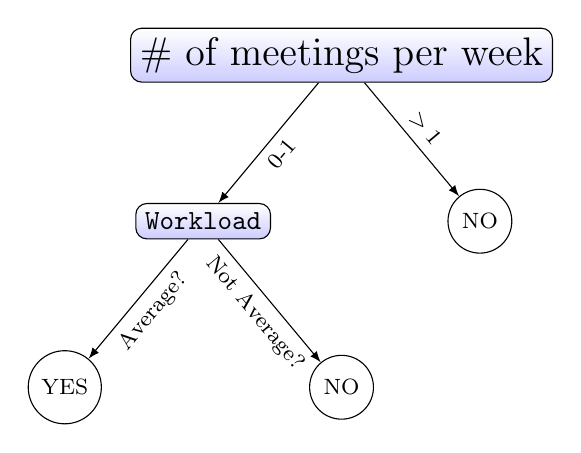
\begin{tikzpicture}
  [
    grow                    = down,
    sibling distance        = 10em,
    level distance          = 6em,
    edge from parent/.style = {draw, -latex},
    every node/.style       = {font=\footnotesize},
    sloped
  ]
  \node [root] {\# of meetings per week}
  child { node [env] {Workload}
    	child { node [dummy] {YES}
        edge from parent node [below] {Average?} }
      child { node [dummy] {NO}
              edge from parent node [above, align=center]
                {}
              node [below] {Not Average?}}
             edge from parent node [below] {0-1} }
    child { node [dummy] {NO}
              edge from parent node [above] {$> 1$} };
\end{tikzpicture}
\end{center}


\subsection{Information gain values:}
At root node, information gains for 
\\$Size = 0.067, Like = 0.031, Workload = 0.061, Meetings = 0.251 \implies Meetings$
\\For depth one node, where \# meetings = 0-1, information gains for 
\\$Size = 0.114, Like = 0.035, Workload = 0.439 \implies Workload$

\subsection{Further splitting:}
For root node's children, \# meetings $> 1$ is not split into $2-3$ and $>3$ because all the entries which fall into these categories are classified in the `No' class.
\\For  Workload's children, the `Average' child has all values as YES(for average workload 3/3) and the `Not average' child has majority NO values(6 out of 8). I chose to merge the light and heavy workload resulting in 6/8 cases being NO. I could have chosen to merge the light workload(1 YES, 1 NO) with either the average or the heavy workload part but both the splits give the same accuracy for the test data.

\iffalse
\begin{table}[h!]
\centering
{\small
\begin{tabular}{| c | l | c | c | c | c | c |}
	\hline
	S.No. & Name  & $\substack{\text{Size of}\\\text{research group}}$ & $\substack{\text{Like the}\\\text{research area?}}$ & $\substack{\text{Average}\\\text{workload?}}$ & $\substack{\text{\# of meetings}\\\text{per week}}$ & $\substack{\text{Good}\\\text{advisor}}$? \\ \hline
	4 & Prof. C. Binns & medium & no  & heavy & $0-1$ & no \\ \hline
	5 & Prof. A. Sinistra & large  & no  & heavy & $0-1$ & no \\ \hline
	6 & Prof. S. Snape & medium & no  & heavy & $0-1$ & yes \\ \hline
	10 & Prof. R. Hooch & medium & no  & light & $0-1$ & no \\ \hline
	12 & Prof. A. P. W. B. Dumbledore & medium & yes & light & $0-1$ & yes \\ \hline
	14 & Prof. H. Slughorn & medium & no  & heavy & $0-1$ & no \\ \hline
	15 & Prof. Q. Quirrell & large  & yes & heavy & $0-1$ & no \\ \hline
\end{tabular}
}
\end{table}
\fi

\end{mlsolution}

\begin{mlsolution}
This is for Question 2

\end{mlsolution}

\begin{mlsolution}
\section*{1. Vacuous constraints:}
\textbf{To prove:} The given optimization problem has the same solutions with and without the constraint:
$\xi_i \geq 0, \text{ for all } i \in [n]$.\newline
\\\textbf{Proof:}
\\We will prove this by contradiction.
\\ Suppose $\hat{\vw},\bc{\hat{\xi_i}}$ are solutions to the optimization problem without the last constraint for some given inputs such that $\hat{\xi_k} < 0$ for at least one $k \in [n]$.
\\ Consider a new proposed solution to the optimization problem $\hat{\vw'},\bc{\hat{\xi'_i}}$ such that 
\\$\hat{\vw'} = \hat{\vw},\  \hat{\xi'_k} = 0 \text{ and } \hat{\xi'_i} = \hat{\xi_i}\  \forall\  i \in [n] \setminus \{k\}.$\newline
\\It is easy to see that the new proposed solution satisfies the constraints that
\\ $\ y^i\ip{\hat{\vw'}}{\vx^i} \geq 1 - \hat{\xi'_i}, \text{ for all } i$. 
\\For $i \neq k$, the constraint is satisfied since we took it $\hat{\xi'_i} = \hat{\xi_i}$ and $\hat{\xi_i}$ is a part of the solution of the initial optimisation problem.
\\For $i = k$, we have 
\\ $\ y^i\ip{\hat{\vw}}{\vx^i} \geq 1 - \hat{\xi_i}\  \because\ \text{it was part of the initial solution} $
\\$\implies y^i\ip{\hat{\vw}}{\vx^i} \geq 1 - \hat{\xi_i}\ $
\\$\implies y^i\ip{\hat{\vw}}{\vx^i} \geq 1\ \because\ \hat{\xi_k} < 0\ $
\\$\implies y^i\ip{\hat{\vw'}}{\vx^i} \geq 1\ \because\  \hat{\vw'} = \hat{\vw} $
\\$\implies y^i\ip{\hat{\vw'}}{\vx^i} \geq 1 - \hat{\xi'_i}\ \because\  \hat{\xi'_k} = 0 $\newline
\\Thus, we have a solution which satisfies all the given constraints AND
\\$\norm{\hat{\vw'}}_2^2 + \sum_{i=1}^n\hat{\xi'_i}^2 < \norm{\hat{\vw}}_2^2 + \sum_{i=1}^n\hat{\xi_i}^2 $.
\\Thus, $\hat{\vw},\bc{\hat{\xi_i}}$ could not have been an optima if $\hat{\xi_k} < 0$ for at least one $k \in [n]$
\\$\implies \text{ for an optimal solution, } \xi_k \geq 0\  \forall\  k \in [n]$

\section*{2. Lagrangian:}
$$\mathcal{L}(\vw,\bc{\xi_i},\valpha,\vbeta) =  \norm{\vw}_2^2 + \sum_{i=1}^n\xi_i^2 + \sum_{i=1}^n\valpha_i (1- \xi_i - y^i\ip{\vw}{\vx^i}) + \sum_{i=1}^n\vbeta_i(-\xi_i)  $$

\section*{3. Dual Problem:}
To get the dual problem, we need to eliminate the primal variables $\vw$ and $\bc{\xi_i}$ from the Lagrangian.

We first take the gradient of $\mathcal{L}$ wrt $\vw$ and equate it to zero.
$$\nabla_\vw\mathcal{L}(\vw,\bc{\xi_i},\valpha,\vbeta) = 0$$
$$\implies 2\vw - \sum_{i=1}^n\valpha_i y^i{\vx^i} = 0  $$
$$\implies \vw = \sum_{i=1}^n\frac{\valpha_i}{2}y^i{\vx^i}$$
After substituting this in the equation for the Lagrangian, we get:
$$\mathcal{L}(\bc{\xi_i},\valpha,\vbeta) = \frac{1}{4}\sum_{i=1}^n \sum_{j=1}^n\valpha_i\valpha_j y^i y^j {\vx^i.}{\vx^j} + \sum_{i=1}^n\xi_i^2 - \frac{1}{2}\sum_{i=1}^n \sum_{j=1}^n\valpha_i\valpha_j y^i y^j {\vx^i.}{\vx^j} + \sum_{i=1}^n\valpha_i (1- \xi_i)  + \sum_{i=1}^n\vbeta_i(-\xi_i)  $$
$$\implies \mathcal{L}(\bc{\xi_i},\valpha,\vbeta) = -\frac{1}{4}\sum_{i=1}^n \sum_{j=1}^n\valpha_i\valpha_j y^i y^j {\vx^i.}{\vx^j} + \sum_{i=1}^n\xi_i^2 + \sum_{i=1}^n\valpha_i (1- \xi_i) + \sum_{i=1}^n\vbeta_i(-\xi_i)  $$
We now take the gradient wrt $\vxi$ and equate it to zero.
$$\nabla_\vxi\mathcal{L}(\vxi,\valpha,\vbeta) = 0$$
$$\implies 2\vxi - \valpha - \vbeta = 0$$
$$\implies \vxi = \frac{1}{2} (\valpha + \vbeta)$$
Substituting this into the equation for Lagrangian, we get
$$\implies \mathcal{L}(\valpha,\vbeta) = -\frac{1}{4}\sum_{i=1}^n \sum_{j=1}^n\valpha_i\valpha_j y^i y^j {\vx^i.}{\vx^j} + \sum_{i=1}^n\frac{1}{4}(\valpha_i+\vbeta_i)^2 + \sum_{i=1}^n\valpha_i  - \sum_{i=1}^n\frac{1}{2}(\valpha_i+\vbeta_i)^2$$
$$\implies \mathcal{L}(\valpha,\vbeta) = -\frac{1}{4}\sum_{i=1}^n \sum_{j=1}^n\valpha_i\valpha_j y^i y^j {\vx^i.}{\vx^j} - \frac{1}{4}\sum_{i=1}^n(\valpha_i+\vbeta_i)^2 + \sum_{i=1}^n\valpha_i$$
Therefore, the dual problem is:
$$ \underset{\valpha,\vbeta \geq 0}{\max} \ \Bigg( -\frac{1}{4}\sum_{i=1}^n \sum_{j=1}^n\valpha_i\valpha_j y^i y^j {\vx^i.}{\vx^j} - \frac{1}{4}\sum_{i=1}^n(\valpha_i+\vbeta_i)^2 + \sum_{i=1}^n\valpha_i \Bigg) $$

\section*{4. Comparision with SVM dual:}
The dual problem for original SVM is:
$$\underset{0 \leq \valpha \leq 1}{\max} \ \Bigg( -\frac{1}{2}\sum_{i=1}^n \sum_{j=1}^n\valpha_i\valpha_j y^i y^j {\vx^i.}{\vx^j} + \sum_{i=1}^n\valpha_i \Bigg)   $$ and the dual for (P1) is:
$$ \underset{\valpha,\vbeta \geq 0}{\max} \ \Bigg( -\frac{1}{4}\sum_{i=1}^n \sum_{j=1}^n\valpha_i\valpha_j y^i y^j {\vx^i.}{\vx^j} - \frac{1}{4}\sum_{i=1}^n(\valpha_i+\vbeta_i)^2 + \sum_{i=1}^n\valpha_i \Bigg) $$
Some important differences between the two duals are:
\begin{itemize}
\item The dual for (P1) involves two sets of Lagrange multipliers $\valpha_i$ and $\vbeta_i$ for $i \in [n]$ whereas the dual for the original SVM problem involves only $\valpha_i$
\item $\valpha$ is bounded on both the sides for the dual of the original SVM problem but it is bounded only on one side for the dual problem of (P1).
\item There is a dependence on $(\valpha_i+\vbeta_i)^2$ in the case of the dual problem for (P1) but in the case of the dual problem for the original SVM problem, there is no dependence of such square terms.
\item There is a lesser dependence on the cross terms $\valpha_i\valpha_j$ in the case of the dual for (P1) when compared to the dual of the original SVM problem.
\end{itemize}

\section*{5. Bonus:}
No, the positivity constraints are not vacuous for the original SVM problem.
\\If we remove the positivity constraint from the original SVM problem, then we might end up with different solutions.
\\For example, consider a solution set in which for some value of $i$, we have $y^i\ip{\vw}{\vx^i} > 1$, with the positivity constraint, we would need $\xi_i = 0$ but if we remove the positivity constraint, then we will have at least one better solution i.e keep everything else the same and make $\xi'_i = 1 - y^i\ip{\vw}{\vx^i}$.


\end{mlsolution}

\begin{mlsolution}
\section*{3.}
For the GD solver, the current iterate $\vw^t$ gives better performance

\end{mlsolution}
					
\end{document}